\documentclass{article}
\usepackage{graphicx,xcolor}
\usepackage{algorithmicx,algorithm}
\usepackage[noend]{algpseudocode}
\usepackage{amssymb,amsmath}
\usepackage{tikz}
\usetikzlibrary{automata, positioning, arrows}

\tikzset{
	->, % makes the edges directed
	>=stealth', % makes the arrow heads bold
	node distance=3cm, % specifies the minimum distance between two nodes. Change if necessary.
	every state/.style={thick, fill=gray!10}, % sets the properties for each ’state’ node
	initial text=$ $, % sets the text that appears on the start arrow
}




\newcommand{\jana}[1]{{\color{magenta} #1}}

\newcommand{\Real}{\mathbb{R}}
\newcommand{\obs}{\mathrm{obs}}
\newcommand{\free}{\mathrm{free}}
\newcommand{\AP}{\Sigma}

\begin{document}

\section{Problem Setup}

Let $X$ be a bounded open subset of $\Real^n$ and let $X_\obs \subset X$ be the obstacle region. $X_\free = X \setminus X_\obs$ is called the obstacle-free space. 

A few more things to define in the standard way:
\begin{itemize}
\item A path
\item A collision-free path
\item A ball
\end{itemize}

Consider a labeling $L: X \rightarrow 2^\AP$ \jana{TODO formalize and assume the labeling induces a partitioning into a finite number of regions}. 

Consider a spec given as an \jana{LTL/sc-LTL?} formula over $\AP$.

The problem is to find \jana{a path/an optimal path?} that satisifes the spec. The problem can be solved using straightforward extension to existing algorithms. \jana{Our contribution is a more efficient procedure that ???}

\section{Solution/Contribution draft}

We get a simulation, we project it to the automaton, see what went wrong (is violated or not satisfied yet), in the next try we aim at spotting where the wrong item can be fixed by a different decision.


\begin{itemize}
	\item Learning a small model from the traces, solving that one, lifting the strategy to the original model.
	\item Looking at what remained to be fullfiled and where in the learnt model this is possible.
	\item For unbounded properties, we have to do this hiearchically and check the progress for subformulas. We can do that, using the labelling from Rabinizer.
\end{itemize}

\begin{algorithm}
	\caption{Basic algorithm}\label{alg:general}
	\begin{algorithmic}[1]
		\State build trivial automaton
		\Repeat\Comment{Start new simulation}
		\Repeat\Comment{Next step in simulation}
		\State \Call{ask}{} automaton for advice which Ap to satisfy next
		\State sample a bit to get that one satisfied
		\Until{sampled all the way to satisfaction of the property or too long}
		\State \Call{learn}{} the automaton using also the new sampled paths
		\Until{sampled all the way to satisfaction of the property (fast enough)}
		
		\Procedure{ask}{}
		\State consider product of the learnt (system) automaton (DFA) and of the property automaton ($\omega$-automaton)
		\State for DFA use shortest path to target
		\State for DBA too
		\State for general ones we might need to non-deterministically choose: which Rabin pair of the DRA? which direction in the NBA?
		\EndProcedure
		\Procedure{learn}{}
		\State automata learning or even probabilistic automata/MDP learning
		\EndProcedure
	\end{algorithmic}
\end{algorithm}



\paragraph{Example 1}
Formulae beyond safety: things like $\varphi=GF(a\wedge Xb)\wedge FG(c\wedge dUe)$ do not even have a deterministic B\"uchi automaton, not to mention a DFA, so how to measure progress is not clear form classical approaches. 
(In DFA one can measure the distance to the accepting state, extensible for B\"uchi - not sure this is done, beyond B\"uchi hard.)
Rabinizer tracks the evolution of both parenthesised expressions and after an $a$ this advises us to go for $b$ althought requirement to be satisfied is still exactly $\varphi$.

\begin{figure}[h]
	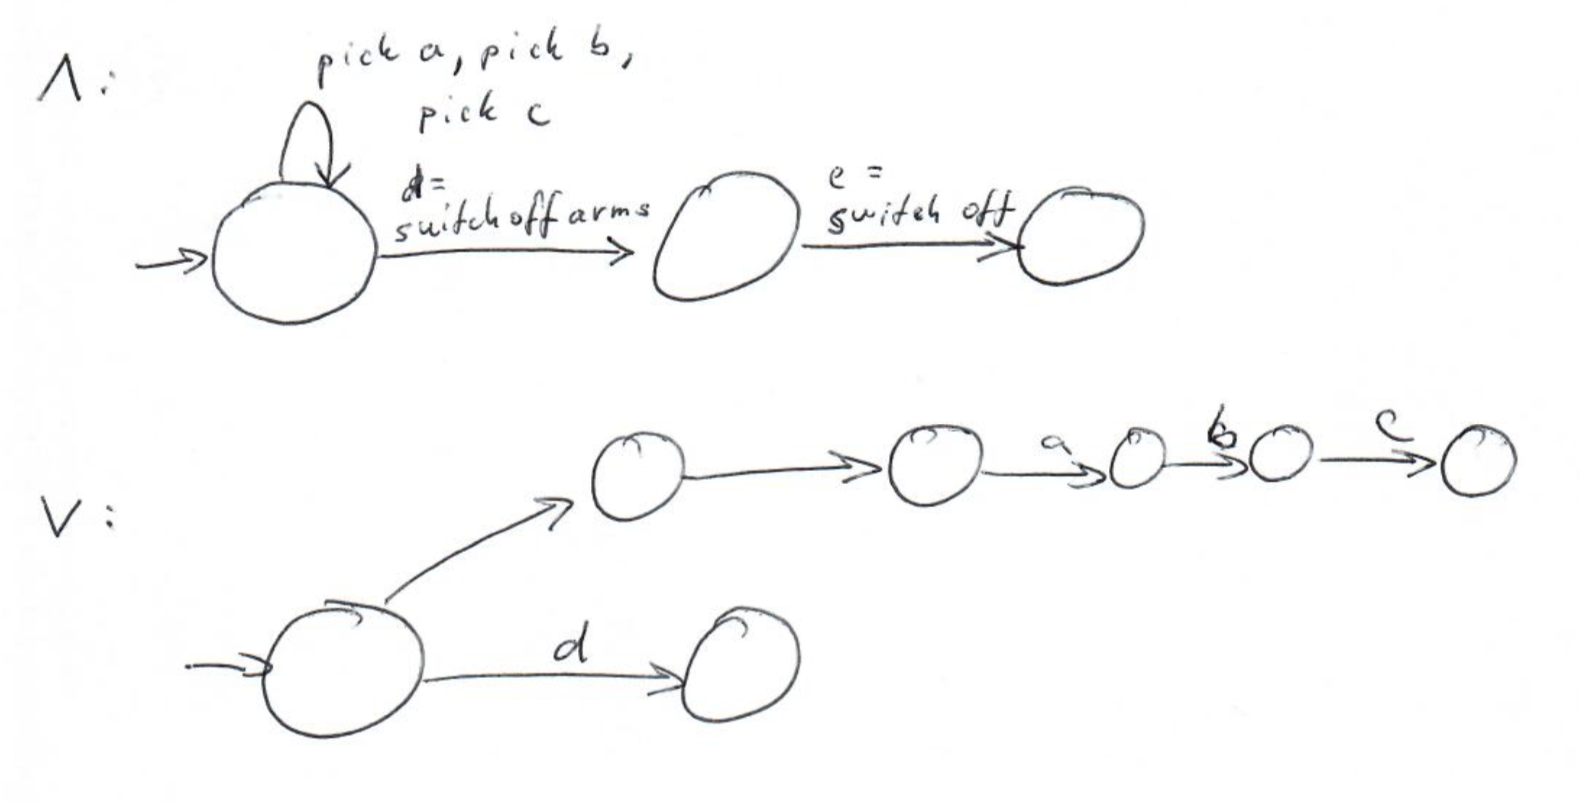
\includegraphics[scale=0.4]{Fig/auto}\caption{Models for the second automata example}
\end{figure}

\paragraph{Example 2}
Write $\alpha\to\beta$ for $\alpha\wedge F\beta$
Within safety, but taking into account the model: $\psi=F(a\to b\to c)\vee F(d\to e)$.
Classical technique (get closer to the accepting state) prefers $d$ 9get to distance 1) over $a$ (distance still 2). 
However, if we see that nothing reasonable comes after $d$, in particular not even an $a$ then we want to try out the first option, too.
To this end we can build a model from learnt traces to see that taking $d$ does not allow for a winning trace.

Similarly, for $\wedge$ instead of $\vee$, getting $d$ is bad at first (no $a$ after $d$, better to stay on spot than to shorten the distance badly).
Seen orders of subsets of $\{a,b,c,d,e\}$ induce a model.
We can make a product with the automaton and then decide there, where to go.

Jana's notes from the call: 
\begin{itemize}
\item State space; partitioned -- we don't know the labels of regions apriori, but if we have a concrete sample, I am able to test whether an atomic proposition holds or not; make sure we formalize this as an assumption; needed: an atomic proposition does not change infinitely many times during a finite time horizon (zeno formulation??)
\jana{Hmm, how can we not have labels of regions apriori, but be able to test samples at all??}
\item Fast finding of A path that satisfies a complex mission. Pre-processing step to Informed RRT* or something like that. Prove that the important properties are maintained beyond reachability.
\jana{Hmm, how can this further guide informed RRT*? I have logically constrained stuff, so the distance is not the metric to guide it now. What is the metric?}
\end{itemize}


\newcommand{\must}{\Rightarrow}
\newcommand{\may}{\rightarrow}
\newcommand{\maynot}{\nrightarrow}
\newcommand{\mustnot}{\nRightarrow}


\begin{algorithm}
	\caption{one simple instantiation}\label{alg:learn}
	\begin{algorithmic}[1]
		\Require ``multi-modal'' transition system $(S,s_0,\must,\may,\maynot,\mustnot)$, $S\subseteq 2^{Ap}$, transition relations disjsoint (generally any quantity $S\times S\to \mathit{OrderedDomain}$, for instance a counter; here just $\{0,1,2,3\}$)
		\Procedure{learn}{transition from $s$ to $s'$}
		\State $t:=(s_1,s_2):=$(Labelling(s),Labelling(s'))
		\If{$t\notin\must$}
		\State add $t$ to $\must$
		\State domainOf Changes$:=\{a\in Ap\mid s_1(a)\oplus s_2(a)\}$
		\For{$s\in S$ agreeing with $s_1$ on domainOf Changes}
		\State \Comment or any other ``neighbourhood'' criterion / one can learn planning-style rules
		\State \Comment(and under some further conditions so that we don't overwrite $\may,\maynot$ back and forth)
		\State add (s,s changed to $s_2$ on domainOfChanges) to $\may$
		\EndFor
		\EndIf
		\State $counter(s_1)++$
		\If {$counter(s_1)>threshold$}
		\For{$s\in S: (s_1,s)\notin$ any relation}
		\State add $(s_1,s)$ to $\maynot$
		\EndFor
		\EndIf
		\EndProcedure
		\State\Comment and $\mustnot$ requires some really good reason to believe there is no transition
		\Procedure Ask{s}
		\State try using the best $\must$-successor or sample long to get an even better $\may$-successor
		\EndProcedure
		\newline
		\State Comments: 
		\State (1) $\maynot$ can be rather written as a $\may$ into ``?'' from where we can go anywhere; ASK tries to win with as few ?'s as possible
		\State (2) $\mustnot$ could be written as $\must$ into a sink ``:-(''
	\end{algorithmic}
\end{algorithm}



\begin{algorithm}
	\caption{Current Implementation: MAIN}\label{alg:current_main}
	\begin{algorithmic}[1]
		\State build trivial automaton
		\Repeat
		\State $adviceBDD$=\Call{ask}{$fromStates$} \Comment{Set of good transitions}
		\State sample a bit to find a transition in $adviceBDD$ ($p \rightarrow q$)
		\State \Call{learn}{$p,q$}
		\State $fromStates = fromStates\vee q$
		\Until{sampled all the way to satisfaction of the property}
	\end{algorithmic}
\end{algorithm}

\begin{algorithm}
	\caption{Current Implementation: LEARN}\label{alg:current_learn}
	\begin{algorithmic}[1]
		\Procedure{learn}{$s_1,s_2$}
		\If{$\Call{getLevel}{s_1,s_2}$ $!=3$}\Comment{Possible levels: 0,1,2,3}
		\State $\Call{setLevel}{s_1,s_2,3}$
		\State $DOC^c=\{a\in APSystem\mid \neg(s_1(a)\oplus s_2(a))\}$\Comment{Used for $restrict$}
		\State $R=restrict(s_1,DOC^c)$\Comment{states smilar to $s_1$}
		\State $newTransitions=R \wedge \neg R' \bigwedge\limits_{a\in DOC^c} a\leftrightarrow a' \wedge level=2$
		\State $productAutomaton $ $\vee= (newTransitions \wedge propertyBDD)$
		\EndIf
		\State $counter(s_1)++$
		\If {$counter(s_1)>threshold$}
		\For{$s\in S: (s_1,s) \wedge productAutomataBDD = false$}
		\State \Call{addTransition} {$s_1,s,1$}
		\EndFor
		\EndIf
		\EndProcedure
	\end{algorithmic}
\end{algorithm}


\begin{algorithm}
	\caption{Current Implementation: ASK}\label{alg:current_ask}
	\begin{algorithmic}[1]
		\Procedure{ask}{$fromStates$}
		\State $finalStates=$\Call{$findFinalStates$}{$productAutomataBDD\wedge fromStates$}
		\State $reachableStates.add(finalStates)$ 
		\State $reachableStates.add(preFinalStates)$\Comment{required for transition acceptance}
		\State $allReachableStates=currentStates[0]$
		\State $i=1$
		\While{$! (\neg allReachableStates \wedge \Call{pre}{allReachableStates}).isZero()$}
			\State $reachableStates.add(\Call{pre}{reachableStates[i]})$
			\State\Comment{add $(i+1)$th element}
			\State $allReachableStates$ $\vee =reachableStates[i+1]$
			\State $i++$
			
		\EndWhile
		\State $fromStates$ $\wedge=allReachableStates$
		\State$toState=\Call{img}{fromStates}\wedge reachableStates[i]$
		\State \Return{$getTransitions(fromStates, toStates)$}
		\EndProcedure
	\end{algorithmic}
\end{algorithm}

\subsection{A mini case study}

Let us consider an office space with several rooms as illustrated in Fig. \ref{fig:office}. There are different objects in the office rooms. For simplicity, let us assume that each of the objects is either a desk (illustrated as a rectangle), or a chair (illustrated as a square), or a waste bin (illustrated as a circle). Consider a fully actuated robot with the initial position $x_0 \in \mathbb{R}^2$. We assume that the robot can recognize if it is close to a certain type of object or landmark in the environment; by close, we mean that the robot's state intersect with the object's/landmark's $\epsilon$-inflation (illustrated as dashed and dotted lines).

The set of atomic propositions is as follows:
\begin{itemize}
\item $\mathit{Room}_1,\ldots,\mathit{Room}_6, \mathit{Hall}$, stand for being in a particular room or in a hallway
\item $\mathit{Desk}$ stands for being close to a desk
\item $\mathit{Chair}$ stands for being close to a chair
\item $\mathit{Bin}$ stands for being close to a bin
\item $\mathit{Corner}$ stands for being close to a corner
\item $\mathit{Wall}$ stands for being close to a wall
\end{itemize}

The specification for the robot's behavior is given by the LTL formula:
$$G F (\mathit{Room}_1 \wedge \mathit{Bin}) \wedge \ldots \wedge G F (\mathit{Room}_6 \wedge \mathit{Bin}).$$

\begin{figure}
\centering
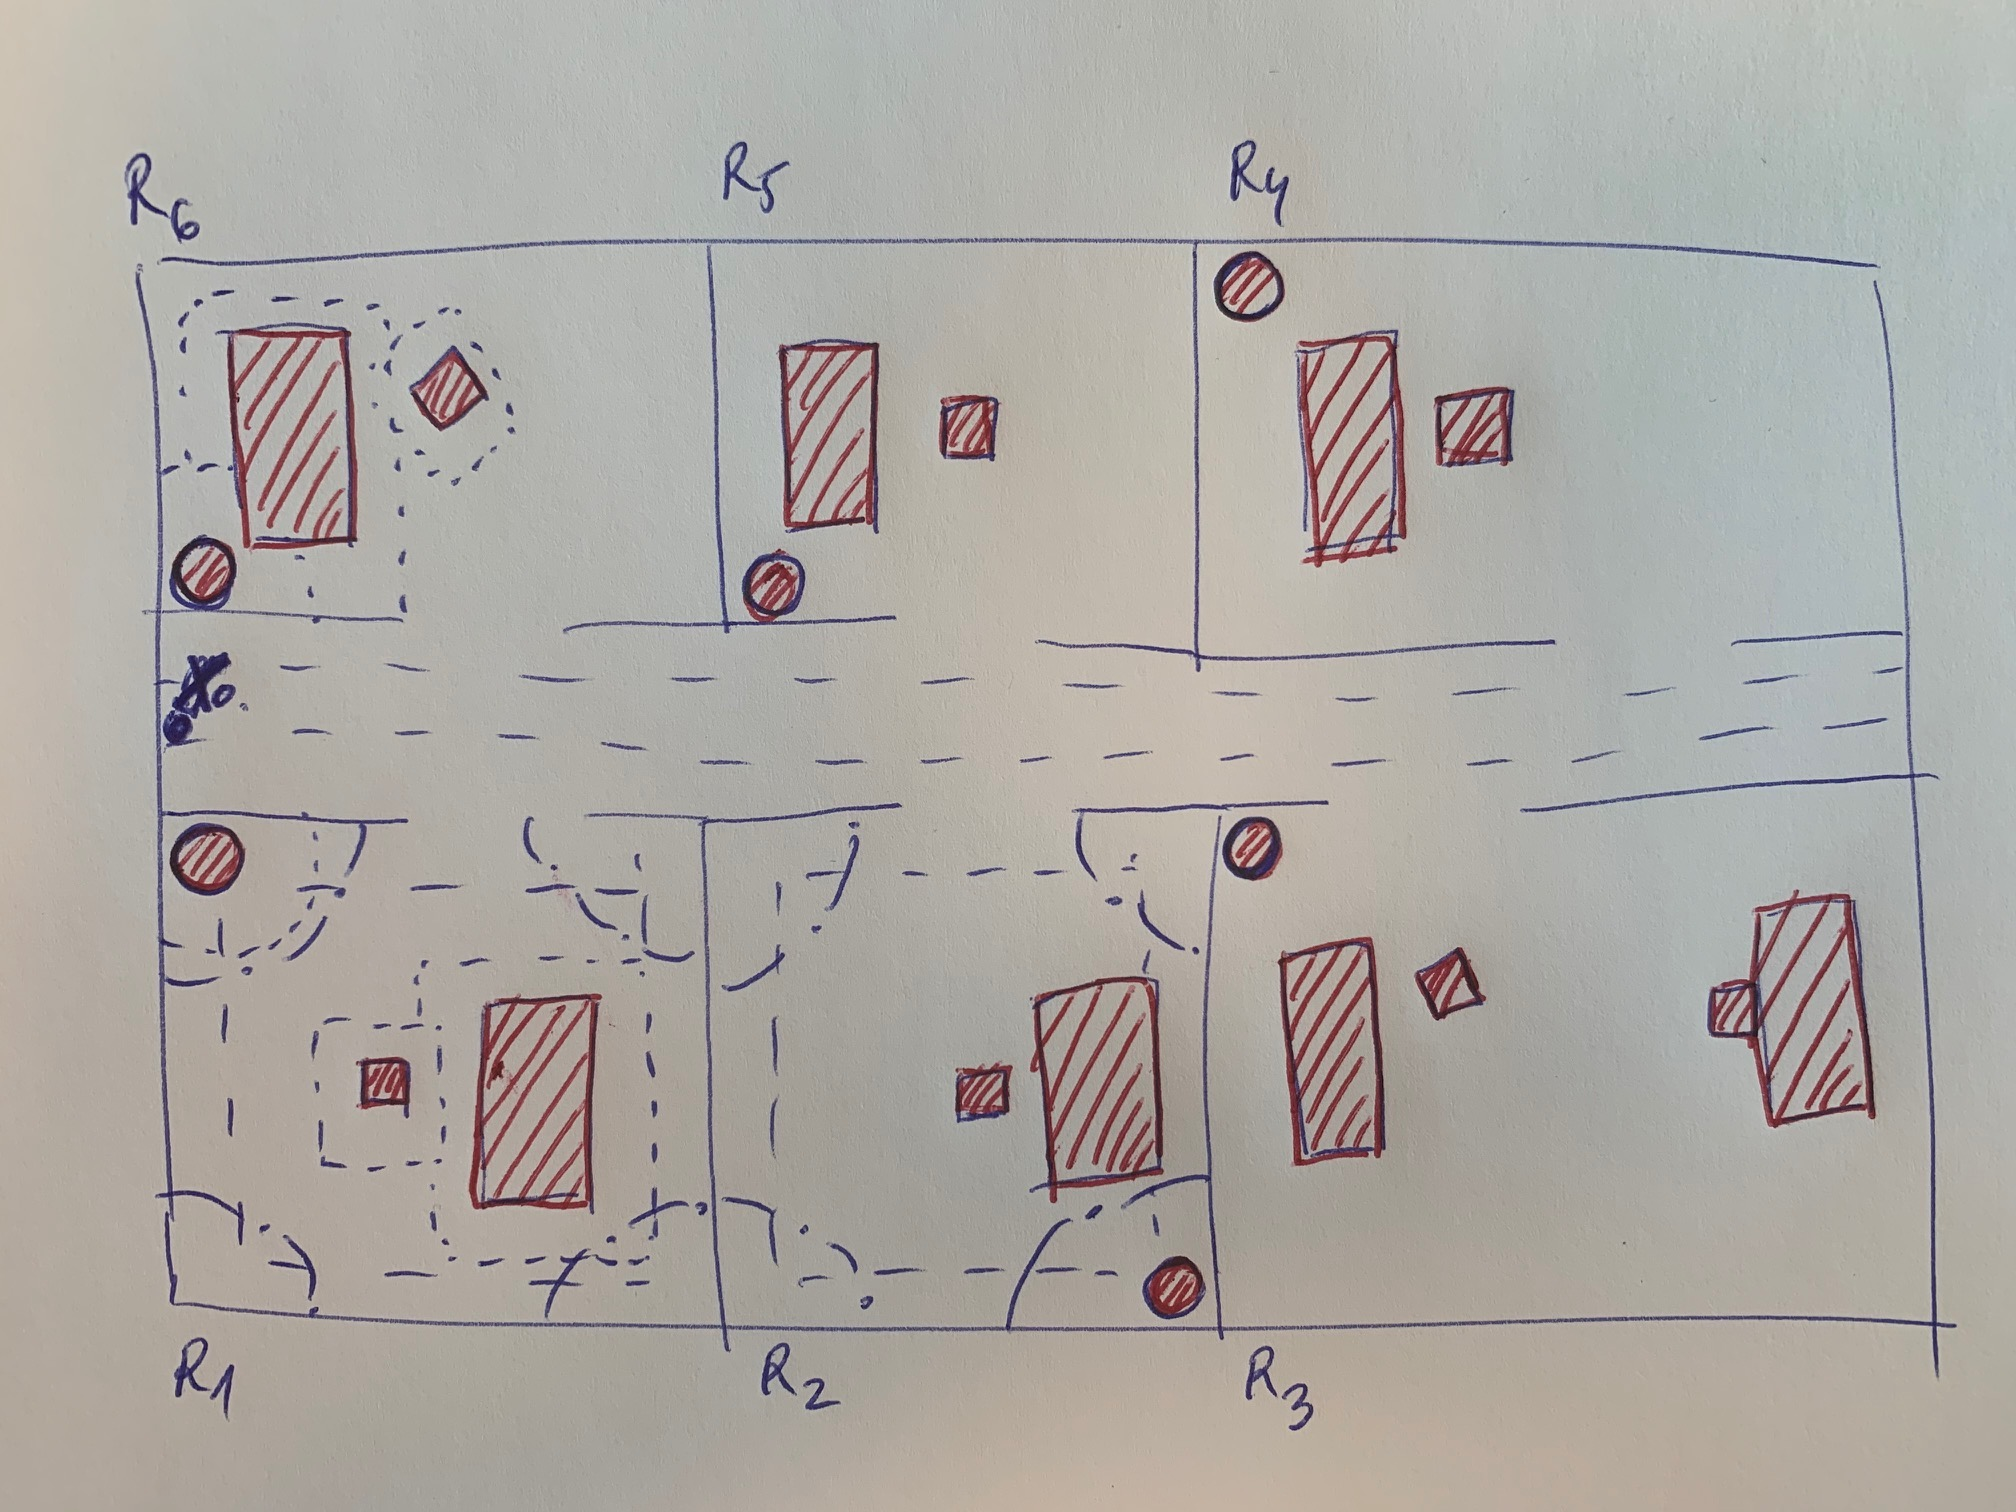
\includegraphics[width=\linewidth]{Fig/small-office} \caption{A mini case study office environment illustration.}
\label{fig:office}
\end{figure}

\subsection{A sample run of the algorithm}


\end{document}
